% Keystone: the Tectonic cache seed (SIM-01, 30 Oct). make-keystone.sh compiles this once with
% TECTONIC_CACHE_DIR inside the bundle, so the study reports compile offline from the first one.
% It loads every package bruceworx_sim.report_source uses and exercises its fonts, tables, colours,
% graphics and pgfplots; TestBruceWorxSimCore checks that it keeps up with the reports.
\documentclass[10pt,a4paper]{article}
\usepackage{iftex}
\ifXeTeX\usepackage{fontspec}\else\usepackage[utf8]{inputenc}\usepackage[T1]{fontenc}\usepackage{lmodern}\fi
\usepackage[margin=20mm]{geometry}
\usepackage{graphicx}
\usepackage{booktabs}
\usepackage{xcolor}
\usepackage{pgfplots}
\pgfplotsset{compat=1.16}
\definecolor{bandA}{HTML}{D91C1C}
\definecolor{bandAmber}{HTML}{F2A007}
\setlength{\parindent}{0pt}\setlength{\parskip}{4pt}
\begin{document}
{\Large\bfseries Seed}\\[2pt]
{\small\color{black!60} Keystone simulation report, \today}
% every size the reports use, in every shape
{\tiny Text \textbf{bold} \textit{italic} \texttt{mono} \textbf{\texttt{monob}} $x_1^2\lambda_{eq} \sigma_{y_{ab}}^{\lambda K_G} \mathrm{d}\psi/\mathrm{d}u$}\par
{\scriptsize Text \textbf{bold} \textit{italic} \texttt{mono} \textbf{\texttt{monob}} $x_1^2\lambda_{eq} \sigma_{y_{ab}}^{\lambda K_G} \mathrm{d}\psi/\mathrm{d}u$}\par
{\footnotesize Text \textbf{bold} \textit{italic} \texttt{mono} \textbf{\texttt{monob}} $x_1^2\lambda_{eq} \sigma_{y_{ab}}^{\lambda K_G} \mathrm{d}\psi/\mathrm{d}u$}\par
{\small Text \textbf{bold} \textit{italic} \texttt{mono} \textbf{\texttt{monob}} $x_1^2\lambda_{eq} \sigma_{y_{ab}}^{\lambda K_G} \mathrm{d}\psi/\mathrm{d}u$}\par
{\normalsize Text \textbf{bold} \textit{italic} \texttt{mono} \textbf{\texttt{monob}} $x_1^2\lambda_{eq} \sigma_{y_{ab}}^{\lambda K_G} \mathrm{d}\psi/\mathrm{d}u$}\par
{\large Text \textbf{bold} \textit{italic} \texttt{mono} \textbf{\texttt{monob}} $x_1^2\lambda_{eq} \sigma_{y_{ab}}^{\lambda K_G} \mathrm{d}\psi/\mathrm{d}u$}\par
{\Large Text \textbf{bold} \textit{italic} \texttt{mono} \textbf{\texttt{monob}} $x_1^2\lambda_{eq} \sigma_{y_{ab}}^{\lambda K_G} \mathrm{d}\psi/\mathrm{d}u$}\par
\section*{Study}
\begin{tabular}{@{}ll@{}}
Young's modulus $E$ & 210000\,MPa, \textit{italic}, \texttt{*STEP, NLGEOM}, \O{} \o{} \dots{}\\
Density & 7850\,kg/m$^3$, $\nu$, $\sigma_y$, $\lambda_1$, $\psi$, $\phi$, $\omega$, $\le$ $\ge$ $\times$ $\cdot$\\
\end{tabular}
\[\sigma_{eq}=\sqrt{\frac{1}{2}\left[(\sigma_1-\sigma_2)^2+(\sigma_3-\sigma_1)^2\right]},\quad
  \left(K+\lambda K_G(\sigma_0)\right)\psi=0,\quad \max(|\sigma_1|,|\sigma_3|)\mbox{ text}\]
\begin{tabular}{@{}rrl@{}}
\toprule Mode & $f$ (Hz) & \\ \midrule
1 & \colorbox{bandAmber!35}{833.7} & \textcolor{bandAmber}{\textbf{in the band}}\\
2 & \textcolor{bandA}{\rule{8mm}{3mm}} & \\
\bottomrule
\end{tabular}
\par\medskip\noindent\fbox{\parbox{0.96\linewidth}{\small\textbf{Note.} Linear buckling is non-conservative.}}
\begin{center}
\includegraphics[width=0.3\linewidth]{seed.png}\\[-2pt]
{\small A render}
\end{center}
\begin{center}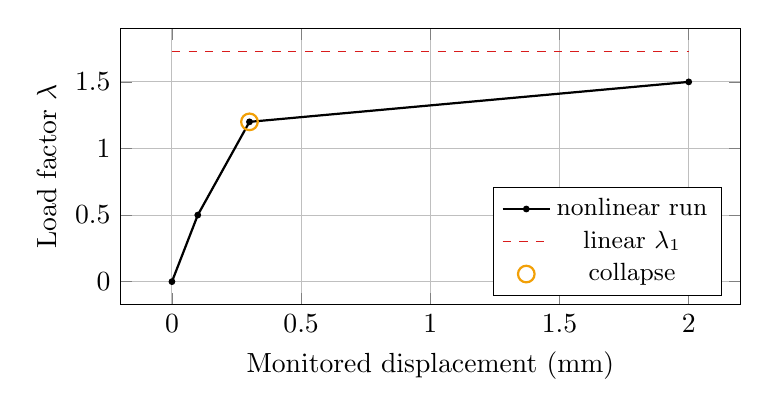
\begin{tikzpicture}
\begin{axis}[width=0.78\linewidth,height=0.42\linewidth,xlabel={Monitored displacement (mm)},
  ylabel={Load factor $\lambda$},grid=major,legend pos=south east,legend style={font=\small}]
\addplot[thick,color=black,mark=*,mark size=0.8pt] coordinates {(0,0) (0.1,0.5) (0.3,1.2) (2,1.5)};
\addlegendentry{nonlinear run}
\addplot[dashed,color=bandA,domain=0:2] {1.73};
\addlegendentry{linear $\lambda_1$}
\addplot[only marks,mark=o,mark size=3pt,color=bandAmber,thick] coordinates {(0.3,1.2)};
\addlegendentry{collapse}
\end{axis}
\end{tikzpicture}\end{center}
\vfill{\small\color{black!60} Static linear analysis: $K u = f$.}
\end{document}
